
\subsection{Формальное определение проблемы: Постановка задачи}
Каждая проблема имеет свою собственную математическую формулировку, поэтому для того, чтобы понять, что мы искали в нашей проблеме, мы описываем ее математическую формулировку.

Прежде всего, набор пользователей, использующих нашу систему, будет обозначаться буквой $U$, а набор элементов - $I$.

Более того, обозначим через R набор рейтингов, записанных в системе, и напишем S набор возможных значений для рейтинга, в этом случае мы будем использовать $S = [1, 5]$. 

Кроме того, мы предполагаем, что любой пользователь u ∈ U для любого элемента $i ∈ I$ может быть не более одного рейтинга и написать $r_{ui}$ этот рейтинг. Чтобы определить подмножество пользователей, которые оценили элемент i, мы используем обозначение $U_{i}$. Аналогично, $I_{u}$ представляет подмножество элементов, которые были оценены пользователем $u$. Наконец, элементы, которые были оценены двумя пользователями $u$ и $v$, то есть $I_{u} \cap I_{v}$, являются важной концепцией в нашей презентации, и мы используем Iuv для обозначения этого понятия. Аналогичным образом, $U{i,j}$  используется для обозначения набора пользователей, которые оценили оба пункта $i$ и $j$.

Двумя наиболее важными проблемами, связанными с системами рекомендаций, являются проблемы с рекомендациями «лучший элемент» и «верхний N». Первая проблема заключается в нахождении для конкретного пользователя u нового элемента $i ∈ I \ I_{u}$, для которого, скорее всего, будет интересен u. Когда рейтинги доступны, эта задача чаще всего определяется как регрессия или ( многоклассовая), задача которой состоит в том, чтобы изучить функцию $f: U \times I \rightarrow  S$, которая предсказывает рейтинг $f\left ( u,i \right )$ пользователя u для нового элемента $i$. Затем эта функция используется, чтобы рекомендовать активному пользователю ua элемент $i^{*}$, для которого оценочная оценка имеет наибольшее значение:

\begin{equation}
i^{*}=\argmax_{j\in I\setminus I_{u}}\\f\left ( u_{a},j \right ).
\label{F:F1}
\end{equation}


\subsection{Метрики оценки}

Точность обычно используется для оценки эффективности метода рекомендации. Как правило, оценки R делятся на обучающий набор Rtrain, используемый для изучения f, и тестовый набор Rtest, используемый для оценки точности прогнозирования. Двумя популярными мерами точности являются средняя абсолютная ошибка $(MAE)$:

\begin{equation}
MAE (f)=\frac{1}{|R_{test}|}\sum_{r_{ui}\in R_{test}}^{n}|f(u,i)-r_{ui})| \\.
\label{F:F2}
\end{equation}

и Root Mean Squared Error $(RMSE)$:


\begin{equation}
RMAE (f)=\sqrt{\frac{1}{|R_{test}|}\sum_{r_{ui}\in R_{test}}^{n} \left ( f(u,i)-r_{ui} \right )^{2} }\\.
\label{F:F3}
\end{equation}


Если рейтинги недоступны, например, если известен только список предметов, приобретенных каждым пользователем, измерение точности прогноза рейтинга невозможно. В таких случаях проблема поиска лучшего предмета обычно превращается в задачу рекомендовать активному пользователю ua список L (ua), содержащий N элементов, которые могут его заинтересовать \cite{topn}. Качество такого метода можно оценить, разбив элементы I на набор $I_{train}$ , используемый для изучения $L$, и тестовый набор $I_{test}$. Пусть $T\left ( u \right )\subset I_{u}\cap I_{test}$ - подмножество тестовых элементов, которые пользователь u нашел релевантным. Если ответы пользователя являются бинарными, это могут быть элементы, которые u положительно оценили. В противном случае, если для каждого пользователя u предоставляется только список приобретенных или доступных элементов, то эти элементы могут использоваться как $T\left ( u \right )$. Выполнение метода затем вычисляется с использованием мер точности и отзыва:

Точность - это соотношение между количеством полученных документов и количеством полученных документов. Таким образом, чем ближе значение точности приближается к нулевому значению, тем больше количество восстановленных документов, которые они не считают релевантными. Если, напротив, значение точности равно единице, то будет понятно, что все восстановленные документы имеют значение.
\\
\begin{equation}
Precision =\frac{1}{\left | U \right |}*\sum_{u\in U}^{  } \left |L\left ( U \right )\cap  T\left ( U \right ) \right |/\left | L\left ( U \right ) \right |\\.
\label{F:F4}
\end{equation}

Отзыв- Это соотношение отражает долю соответствующих документов, восстановленных, по сравнению с общим количеством документов, которые имеют отношение к базе данных, независимо от того, были ли они восстановлены или нет.
\begin{equation}
Recall =\frac{1}{\left | U \right |}*\sum_{u\in U}^{  } \left |L\left ( U \right )\cap  T\left ( U \right ) \right |/\left | T\left ( U \right ) \right |\\.
\label{F:F5}
\end{equation}



\begin{figure}[h]
  \centering
  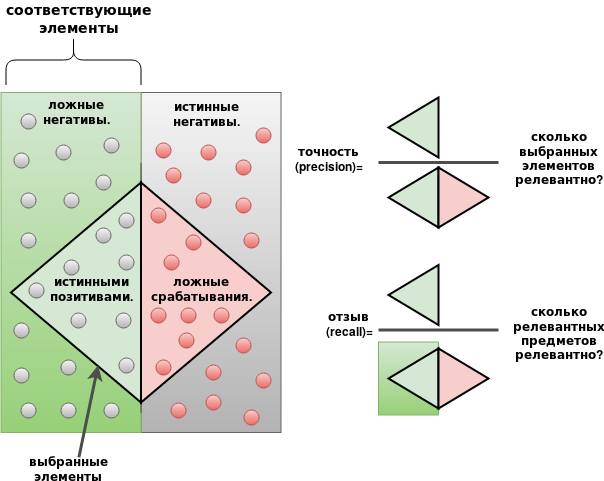
\includegraphics[scale=0.55]{recall.png}
  \caption{Точность и отзыв.}
  \label{image:scheme7}
\end{figure}



Недостатком этой задачи является то, что все элементы списка рекомендаций $L\left ( u \right )$ считаются одинаково интересными для пользователя $u$. Альтернативная настройка, описанная в \cite{topn}, состоит в изучении функции $L$, которая отображает каждого пользователя $u$ в список $L\left ( u \right )$, где элементы упорядочены по своей «интересности» на $u$. Если тестовый набор создается случайным образом, для каждого пользователя u, одного элемента iu Iu, производительность $L$ может быть оценена с помощью Среднего Взаимного $Хит-Ранга (ARHR)$:


\begin{equation}
ARHR(L)=\frac{1}{\left | U \right |}*\sum_{u\in U}^{  } \frac{1}{rank(i_{u},L(u))}\\.
\label{F:F6}
\end{equation}

где $rank \left ( I_{u},L\left (u  \right ) \right )$ - ранг элемента $RHR(L)$ $I_{u}$ в $L\left (u  \right )$, равный $\infty$, если $I_{u}\notin  L_{u}$.
\textit{«Вот строятся математические формулы»}\\



Прежде чем приступать к изучению алгоритмов, мы изучим набор метрики \cite{topn}. Как правило, набор квалификаций делится на два подмножества: «ET» - это подмножество квалификаций, которые будут использоваться в качестве учебного набора, то есть для составления прогнозов; С другой стороны, «EP» будет подмножеством, которое будет сравниваться с соответствующими прогнозами для оценки эффективности рекомендаций.




\newpage
\section{Архитектура и подходы рекомендательная системы}

\begin{figure}[h]
  \centering
  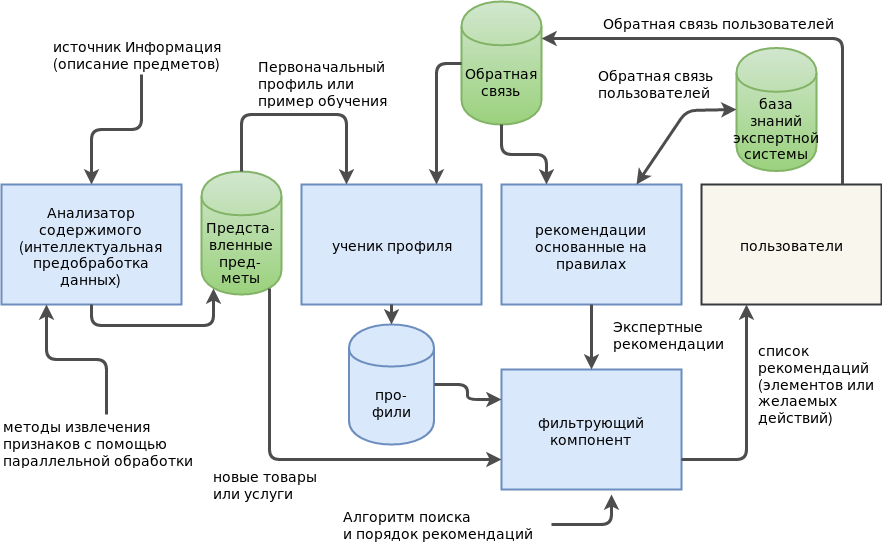
\includegraphics[scale=0.55]{struct_sys.png}
  \caption{ССхема, выбранная для выбранной рекомендательная системы}
  \label{image:scheme6}
\end{figure}

\subsection{Архитектура}
Архитектура системы предусматривает несколько экземпляров, которые обмениваются информацией, в основном отзывами пользователей и ссылкой на предложения продуктов и услуг. Самое подходящее, что каждый город или район могут управлять своей информацией. Данные пользователя являются частью конфиденциальной информации, которая не является общей.

\subsection{Обратная связь}
Обратная связь - это самая важная информация об этой архитектуре, выбор пользователя служит не только для совместной работы с алгоритмами для разработки рекомендаций, но также дает информацию об использовании и обычаях каждого региона. В свою очередь, эта информация служит для сравнения окрестностей с точки зрения разных вариантов по каждой теме и для предоставления наилучших предложений.

\subsection{Передача данных между экземплярами}
Для обмена информацией между экземплярами рассматриваются две альтернативы, первая заключается в том, что каждая система рекомендаций является частью «архитектуры HLA высокого уровня» \cite{hla}, которая делится данными и синхронизирует информацию с другими системами через «Runtime инфраструктуры RTI» \cite{rti} и действовать в симуляции. Вторая - архитектурно-ориентированная сервис-ориентированная архитектура (SOA), где обмен информацией распределяется между службами в архитектуре с низким уровнем связи, используя веб-службы RESTFul. Из-за сложности присущего слоя первого варианта выбирается архитектура API Rest.

\subsection{Защита данных и уведомление}
Информация в данных профиля локальна и не используется. Эти данные принадлежат пользователям, которые живут по соседству. Система предупреждений и уведомлений для пользователей о новых продуктах и мероприятиях или просто рекомендации предупреждает о событиях. Сама система может считаться сервисом или набором услуг.

\subsection{Свободное и открытое программное обеспечение}
Набор функциональных возможностей формирует группу (анализатор данных, менеджер профилей, фильтрацию) и данные: профили пользователей, отзывы и совместную поддержку (данные, планы и правила). Первое не разделяется, а два других.

\newpage
\subsection{Подходы «Content-Based»}
"Content-based" фильтрация предоставляет альтернативные элементы, которые контекстуализируются для просматриваемого элемента.

Система сопоставляет атрибуты элемента, просмотренного с атрибутами других элементов, для генерации рекомендаций, чтобы найти те атрибуты, которые относятся к определенному продукту.

Этот подход основан на описаниях пользовательских предпочтений и предметов, которые они просмотрели или приобрели в прошлом.


\begin{enumerate}
\item «Content-based» Фильтрация  предоставляет альтернативные элементы, которые контекстуализируются для просматриваемого элемента.
\item Система сопоставляет атрибуты элемента, просмотренного с атрибутами других элементов, для генерации рекомендаций, чтобы найти те атрибуты, которые относятся к определенному продукту.
\end{enumerate}

\begin{figure}[h]
  \centering
  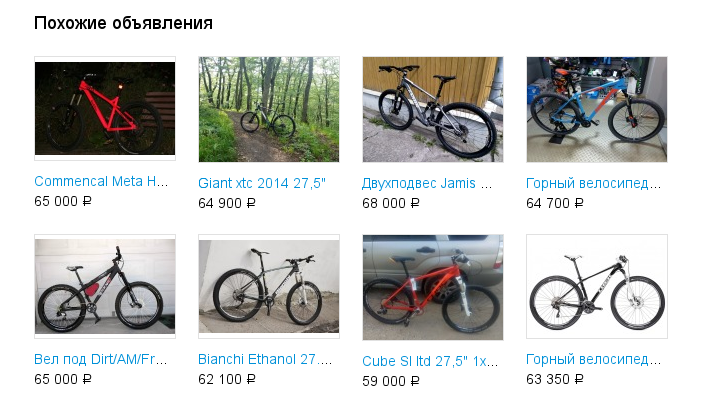
\includegraphics[scale=0.55]{bicis.png}
  \caption{Аналогичные элементы, как выбор пользователя}
  \label{image:scheme5}
\end{figure}


\subsection{TD/IDF}
Чтобы найти эти атрибуты, более релевантные для определенного элемента, мы используем методы «NLP», такие как «TF/IDF».

Модель векторного пространства на основе ключевых слов
Наиболее "content-based" систем рекомендаций на основе контента используют относительно простые модели поиска, такие как сопоставление ключевых слов или модель векторного пространства (VSM) с базовым взвешиванием TF-IDF. VSM представляет собой пространственное представление текстовых документов. В этой модели каждый документ представлен вектором в n-мерном пространстве, где каждый размер соответствует термину из общей лексики данного набора документов.

Формально каждый документ представляется в виде вектора весовых коэффициентов, где каждый вес указывает степень ассоциации между документом и термином. Пусть $D=  d_{1},d_{2},...,d_{n}$ обозначает набор документов или corpus, а $T=  t_{1},t_{2},...,t_{n}$ - словарь, т. Е. набор слов в корпусе. T получается путем применения некоторых стандартных операций обработки естественного языка, таких как токенизация, удаление стоп-слов и создание. Каждый документ d j представлен как вектор в n-мерном векторном пространстве, поэтому  $d_{j}=  w_{1,j},w_{2,j},...,d_{n,j} $, где $w_{k,j}$ - вес для члена $t_{k}$ в документе $d_{j}$.

Представление документов в VSM вызывает два вопроса: взвешивание терминов и измерение сходства вектора признаков. Наиболее часто используемая терминологическая Типосхема взвешивания, TF-IDF (временная частота-обратная документальная частота), основана на эмпирических наблюдениях.


\begin{itemize}
    \item редкие термины не менее важны, чем частые термины (предпосылка IDF).
    \item множественные появления термина в документе не менее важны, чем отдельные случаи (предположение TF).
    \item длинные документы не являются предпочтительными для коротких документов (предположение о нормализации).
\end{itemize}


Другими словами, термины, которые часто встречаются в одном документе (TF =term-frequency), но редко в остальной части корпуса (IDF = частота обратного документа), больше вероятно, будут иметь отношение к теме документа. Кроме того, нормализация полученных весовых векторов предотвращает получение более длинных документов с большей вероятностью извлечения. Эти предположения хорошо иллюстрируются функцией TF-IDF:




\begin{equation}
tdidf\left ( t,d,D \right )=tf(t,d)*idf(t,D)\\.
\label{F:F7}
\end{equation}

\begin{equation}
tf(t,d)=0.5+0.5*\frac{f_{t,d}}{max\left \{ f_{t^{'},d}:t^{'}\in d \right \}}\\.
\label{F:F8}
\end{equation}

\begin{equation}
\left. \begin{matrix}
td \;\;  is\; high\\ 
idf\; is \;low
\end{matrix} \right \} \Rightarrow High\: TD/IDF\\.
\label{F:F9}
\end{equation}
\newpage
\subsection{Архитектура «Content-Based» систем}

\begin{figure}[h]
  \centering
  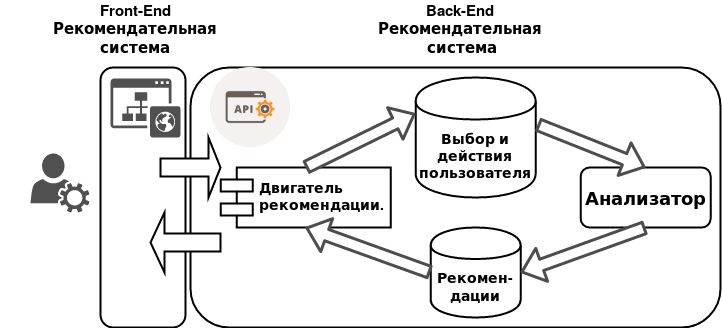
\includegraphics[scale=0.55]{content.png}
  \caption{Структура системы рекомендаций}
  \label{image:scheme8}
\end{figure}
Три отдельных модуля «Анализатор содержимого», «ученик профиля» и «Фильтрующий компонент», которые отвечают за процесс рекомендации, используя надлежащие методы для представления элементов и создания профиля пользователя, а также некоторые стратегии для сравнения профиля пользователя с представлением элемента.

Анализатор содержимого
В базе данных мы можем хранить данные в таблицах, и нетрудно получить информацию, использующую, например, команды SQL, но когда данные не имеют структуры (например, opioions, размещенные на веб-сайтах, веб-страницах, новостях, описаниях продуктов и т. Д.), Поступающих из разных источников в более подходящий источник восстановления через задачи предварительной обработки в другом, чтобы извлечь структурированную релевантную информацию. Это основная задача анализатора контента, но она является высокопоставленным потребителем, технология использует новые технологии для таких задач, как Apache Hadoop или Spark, которые хранят информацию в «озерах данных» \cite{lakes} больше полезной для обработки больших данных, в режиме реального времени аналитика и машинное обучение для лучшего решения.


Элементы данных анализируются с помощью методов извлечения признаков, чтобы переместить представление позиции из исходного информационного пространства в целевое (например, веб-страницы, представленные как векторы ключевых слов).

Первым шагом процесса рекомендации является тот, который выполняется «Анализатором содержимого», который обычно заимствует методы из систем поиска информации \cite{retrieve}. Описание описаний, исходящих из Источника информации, обрабатывается с помощью анализазаторского содержимого, которое извлекает функции (ключевые слова, n-граммы, концепции и т. Д.) Из неструктурированного текста для создания структурированного представления элемента, хранящегося в репозитории «Представленные элементы».

Эта предварительно обработанная информация представляет собой вход для модулей «Изучение профиля» и «фильтрующий компонент».

Модуль «Изучение профиля» собирает данные данных пользователя и использует методы машинного обучения для создания профиля пользователя, чтобы иметь возможность выводить модель интересов пользователей, начиная с предметов, которые нравились или не нравились в прошлом. Также модуль реализует метод обратной связи обратной связи \cite{retrieve}, в котором метод обучения объединяет векторы положительных и отрицательных примеров в векторе прототипа, представляющем профиль пользователя.

\begin{figure}[h]
  \centering
  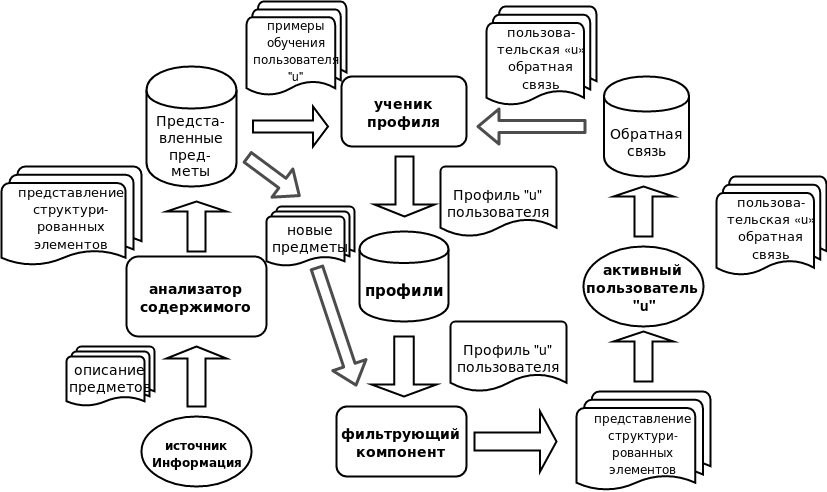
\includegraphics[scale=0.55]{hla.png}
  \caption{Архитектура «Content-Based» систем}
  \label{image:scheme9}
\end{figure}

Модуль «Фильтрующий компонент» использует профиль пользователя, чтобы предлагать соответствующие элементы, сопоставляя представление профиля с параметром, рекомендуемым для элементов. Результатом является суждение, сравнивая предпочтения в представлении элемента с элементами в пользовательских предпочтениях (хранящихся в профиле пользователя). Результат в ранжированном списке потенциально интересных предметов. Согласование выполняется путем вычисления сходства косинусов между вектором прототипа и векторами предметов.

Пользовательские вкусы обычно меняются со временем, поэтому предпочтения должны поддерживаться и предоставляться «Изучение профиля», чтобы автоматически обновлять профиль пользователя. Когда пользователи сообщают о своем удовлетворении или неудовлетворенности выбранными позициями, обратная связь заключается в том, что процесс обучения снова выполняется в новом наборе тренировок, и полученный профиль адаптирован к обновленным интересам пользователей.
\subsection{Создание профиля и отзывов в явных оценках}

Чтобы создать пользовательский профиль, должен быть определен обучающий набор для пользователя. Учебный набор представляет собой пары $⟨i_{k}, r_{k}⟩$, где $r_{k}$ - это рейтинг, предоставляемый ua в представлении элемента I k.

Учитывая набор позиций, помеченных рейтингом, «Изучение профиля» применяет контролируемые алгоритмы обучения для создания предсказательной модели, которая хранится в «репозитории профилей» для последующего использования «фильтрующим компонентом».

Чтобы создать и обновить профиль активного пользователя ua (пользователя, для которого должны быть предоставлены рекомендации), ее реакция на элементы собирается каким-то образом и записывается в репозиторий «Обратная связь»\cite{retrieve}.

\subsection{Определение, преимущества и недостатки}
\subsection{Алгоритмы «Content-Based»}

\subsection{Построение «Рекомендательная система»}
\subsection{Анализ требований}
\subsection{Анализ и разработка решения}


\subsection{Подходы «Коллаборативная фильтрация»}


Совместная фильтрация - это метод автоматического прогнозирования (фильтрации) об интересах пользователя путем сбора предпочтений или информации о вкусе у других пользователей (сотрудничающих).


Он предполагает, что если у человека А есть такое же мнение, как у человека в вопросе, у А более вероятно, что мнение Б будет по другому вопросу, чем у случайно выбранного человека.

\begin{figure}[h]
  \centering
  
\includegraphics[scale=0.65]{others.png}
  \caption{Предложения от другого выбора пользователя}
  \label{image:scheme10}
\end{figure}

Типы: Пользователь к пункту: лучшее преобразование, но сложнее вычислить
Элемент к пункту: меньше времени зависит, но менее эффективно.

Альтернативные наименьшие квадраты или ALS являются более распространенным алгоритмом CF и являются методом матричной факторизации.
Он разлагает матрицу оценок пользовательских позиций на две части:


\begin{itemize}
    \item Пользовательская матрица с ней скрытые факторы (характеристики).
    \item Транспонирование матрицы элементов со своим скрытым фактором.
\end{itemize}

\begin{figure}[h]
  \centering
  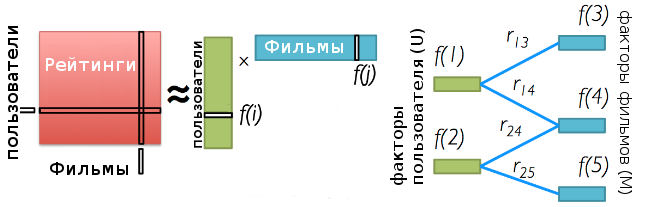
\includegraphics[scale=0.7]{descompo.png}
  \caption{Разделить рейтинги «пользовательский элемент»}
  \label{image:scheme11}
\end{figure}

В основном существуют два типа систем рекомендаций: «на основе контента» и «совместная фильтрация». В системах рекомендаций «на основе контента» система учитывает только квалификацию (неявную или явную), которую пользователь, получивший рекомендацию, сделал на некоторых элементах заранее. На основе этих квалификаций прогнозируется рейтинг, который пользователь предоставит остальным элементам, составляющим систему, и пользователю с наивысшим прогнозируемым значением предлагается пользователю.

Системы рекомендации типа «Коллаборативная фильтрация» наиболее часто используются в наши дни, поскольку с учетом квалификации всех пользователей системы могут предлагаться более разнообразные рекомендации, но с учетом оценки пользователя.

Основная идея заключается в том, что рейтинг «$u$» для нового элемента «$i$», скорее всего, будет похож на рейтинг другого пользователя «$v$», если «$u$» и «$v$» оценили другие элементы аналогичным образом. Аналогичным образом, «u», вероятно, будет оценивать два элемента «$i$» и «$j$» аналогичным образом, если другие пользователи дали аналогичные рейтинги этим двум элементам.

Начнем с примера: «Amazon» \cite{amazon} использует систему рекомендаций для совместной фильтрации, чтобы предлагать рекомендации своим пользователям. Первоначально, когда пользователь является новым, он предлагает рекомендацию «по отдельности», предлагающую рекомендации, основанные на элементе, который пользователь недавно видел. То есть, если пользователь посетил ссылку в «ремонте дома», связанную с «Живописью для белых фасадов», следующая вещь, которую система порекомендует, будет другими типами «покрытие для фасадов домов» или «краска для внешней», ». Таким образом, это позволяет избежать холодного начала, с которым страдают системы рекомендаций, когда у них мало информации.

Позже, когда система получает больше информации о пользователе (он проявляет интерес к большему количеству продуктов или предметов) и может избежать холодного запуска, он уже использует систему рекомендаций «пользователь для пользователя», то есть он ищет пользователя текущие среди остальных наиболее похожих, те, кто видел или купил те же предметы. Из интересов этих пользователей предлагаются рекомендации к текущему.

Он также использует глобальные алгоритмы факторизации, то есть сравнивает несколько характеристик для каждого элемента и присваивает им вес, чтобы впоследствии иметь возможность вычислять сходство между элементами с учетом нескольких факторов и определять приоритеты тех, для которых пользователь проявляет больше интереса.

Ниже приведены два алгоритма совместной фильтрации с различными способами получения прогнозов:

\subsection{Определение, преимущества и недостатки}

Сильные стороны, которые выделяются в алгоритме, делают это как с начала операции, в то время как система растет экспоненциально, надежность, эффективность и стоимость работы поддерживаются.

Простота: этот метод относительно прост для реализации и интуитивно понятен, и только количество соседей, используемых в предсказании, должно быть установлено как параметр. Лучше начать с алгоритма, который мы можем понять.

Обоснованность: дать доверие к результатам обоснование в необходимом. Например, в рекомендации, основанной на элементах, список соседних элементов, а также рейтинги, предоставленные пользователем этим элементам, могут быть представлены пользователю в качестве обоснования для рекомендации. Кроме того, пользователи по соседству могут понять значимость рекомендаций, а также служить основой для интерактивной системы, в которой пользователи могут выбирать соседей, для которых большее значение должно быть дано в рекомендации.

Эффективность. Одной из сильных сторон систем, основанных на окрестности, является их эффективность. В отличие от подхода, основанного на модели, он не требует дорогостоящих этапов обучения, а ближайших соседей можно предварительно вычислить в автономном режиме, обеспечивая почти мгновенные рекомендации. Более того, хранение этих ближайших соседей требует очень небольшой памяти, что делает такие подходы масштабируемыми для приложений, имеющих миллионы пользователей и элементов. Нет необходимости иметь большую инфраструктуру.

Стабильность: Еще одно полезное свойство этого подхода заключается в том, что новые пользователи, элементы и рейтинги могут быть добавлены, а система будет стабильной, не нужно тренироваться снова и когда новые оценки будут введены для нового элемента, только сходство между этим элементом и которые уже в системе должны быть вычислены.


\subsection{Алгоритмы «Коллаборативная фильтрация»: Алгоритм соседнего K}


Алгоритм соседнего K является одним из наиболее употребительных в библиографии, так как это очень простой алгоритм с достаточно точными результатами. Проблема возникает, когда вы намерены использовать ее в очень большой системе, поскольку масштабируемость не является одним из ее преимуществ: за счет увеличения объема данных количество операций, необходимых для рекомендации, значительно увеличивается. Существуют две версии этого алгоритма: алгоритм соседнего пользователя «пользователь к пользователя» и алгоритм соседнего элемента K «элемент к элементу»; в обоих случаях фиксированное число соседей может быть заменено порогом подобия, чтобы выбирать только соседей, которые достигают определенного уровня подобия.

Алгоритм соседнего пользователя K "пользователю"
Эта версия алгоритма основана на идее, что аналогичные пользователи будут одинаково квалифицировать один и тот же элемент. Он состоит из трех этапов:



\begin{enumerate}
	\item Используя выбранную меру подобия, строится набор соседнего K целевого пользователя $a$. Соседние $K$ будут теми, для которых большее сходство получается с пользователем $a$.
	\item Как только пользователи $K$, наиболее близкие $к$ пользователю (соседи), уже получены, чтобы вычислить предсказание этого пользователя для элемента $i$, функция агрегации применяется $к$ рейтингам, которые соседние $K$ сделали на пункт $i$.
	\item Чтобы получить $n$ лучших рекомендаций, мы выбираем $n$ элементов, которые обеспечивают пользователю большее удовлетворение в соответствии с прогнозами.
\end{enumerate}


Этот подход обеспечивает хорошие результаты с достаточно заполненной БД, но когда пользователь не выдал много рейтингов, трудно найти достаточно похожих соседей, и происходит так называемый холодный старт.

Он также должен иметь дело с проблемой вышеупомянутой масштабируемости, поскольку для того, чтобы предлагать рекомендации для пользователя, его подобие с каждым из пользователей системы должно быть рассчитано, что-то с очень высокой вычислительной стоимостью.

Алгоритм соседнего элемента $K$ "элемент $к$ элементу"
Версия «по отдельности» алгоритма значительно снижает проблему малой масштабируемости. В этом случае соседи вычисляются для каждого элемента и сохраняются для использования при расчете прогнозов. Эта информация устарела, но она менее чувствительна к хранению неточной информации об элементах, чем о пользователях.


Этапы этого подхода:
\begin{enumerate}
	\item Определите q соседних элементов каждого элемента системы.
	\item Для каждого элемента $i$, не оцененного целевым пользователем a, вычислить прогноз, основанный на оценки, которые он сделал в отношении соседей $i$.
	\item Выберите $n$ лучших рекомендаций для пользователя a из прогнозов шага выше.
\end{enumerate}


